\chapter{บทนำสู่จุลชีววิทยาการเกษตร}
\label{ch:intro}

\begin{keyconcept}[แนวคิดสำคัญของบทที่ 1]
จุลชีววิทยาการเกษตร\index{จุลชีววิทยาการเกษตร (Agricultural Microbiology)} (Agricultural Microbiology) เป็นศาสตร์บูรณาการที่ศึกษาบทบาท ความหลากหลาย และกิจกรรมทางชีวเคมีของประชากรจุลินทรีย์ในระบบนิเวศเกษตรกรรม ทั้งในดิน น้ำ พืช สัตว์ และผลผลิตหลังการเก็บเกี่ยว จุลินทรีย์ทำหน้าที่เป็นตัวขับเคลื่อนหลักในวัฏจักรชีวธรณีเคมี การตรึงธาตุอาหาร การควบคุมศัตรูพืชโดยชีววิธี และการสร้างความสมบูรณ์ของโครงสร้างดิน การนำเทคโนโลยีสารสนเทศ การวิเคราะห์ข้อมูลขนาดใหญ่ และปัญญาประดิษฐ์\index{ปัญญาประดิษฐ์ทางการเกษตร (Agri-AI)} (AI) เข้ามาผสานกับองค์ความรู้ด้านไมโครไบโอมดิน\index{ไมโครไบโอมดิน (Soil Microbiome)} กำลังเปลี่ยนผ่านระบบเกษตรกรรมแบบดั้งเดิมสู่เกษตรกรรมแม่นยำสูง (Precision Agriculture) และความมั่นคงทางอาหารอย่างยั่งยืน
\end{keyconcept}

\begin{figure}[ht]
    \centering
    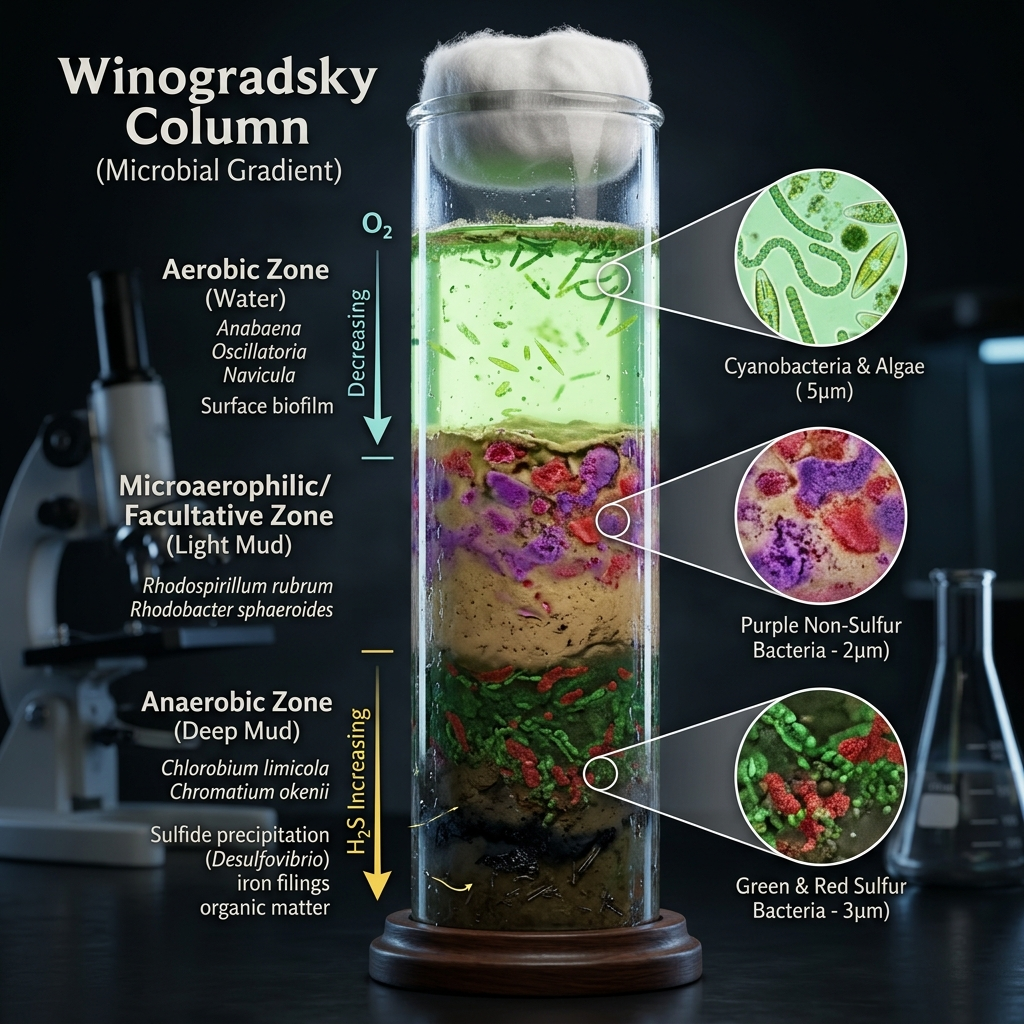
\includegraphics[width=0.85\textwidth]{assets/ch01_winogradsky_column.png}
    \caption{แบบจำลองสามมิติของ Winogradsky Column แสดงการจำแนกชั้นจุลินทรีย์ตามความลาดชันของความเข้มข้นออกซิเจนและไฮโดรเจนซัลไฟด์ ตั้งแต่ชั้นออกซิเจนสูงด้านบนจนถึงชั้นไร้ออกซิเจนที่มีการสะสมซัลไฟด์เข้มข้นด้านล่าง}
    \label{fig:ch01_winogradsky}
\end{figure}

\section*{วัตถุประสงค์การเรียนรู้ประจำบท}
เมื่อศึกษาบทเรียนนี้จบแล้ว นักศึกษาสามารถ:
\begin{enumerate}
    \item อธิบายขอบเขต ความหมาย และปฏิสัมพันธ์หลักของจุลินทรีย์ในระบบนิเวศการเกษตรได้อย่างถูกต้อง
    \item สรุปวิวัฒนาการทางประวัติศาสตร์ การค้นพบครั้งสำคัญ และคุณูปการของนักบุกเบิกจุลชีววิทยาการเกษตร
    \item วิเคราะห์การแบ่งชั้นทางชีวเคมีและสมดุลรีดอกซ์ในแบบจำลองคอลัมน์วิโนกราดสกี (Winogradsky Column)
    \item คำนวณอัตราการเติบโตจำเพาะของจุลินทรีย์ในดินด้วยแบบจำลองจลนศาสตร์ของโมโนด์ (Monod Kinetics)
    \item ประเมินความสำคัญของไมโครไบโอมต่อการขับเคลื่อนเกษตรกรรมยั่งยืนและการฟื้นฟูดินในยุคดิจิทัล
\end{enumerate}

\section{ขอบเขตและความสำคัญของจุลชีววิทยาการเกษตร}

จุลชีววิทยาการเกษตรเป็นสหวิทยาการขั้นสูงที่เชื่อมประสานองค์ความรู้จากวิทยาศาสตร์ดิน (Soil Science) สรีรวิทยาของพืช (Plant Physiology) ชีวเคมี พันธุศาสตร์ระดับโมเลกุล และวิทยาการคำนวณ เพื่อทำความเข้าใจบทบาทของจุลินทรีย์ในมิติต่าง ๆ โดยจำแนกออกเป็น 4 ขอบข่ายหลักได้แก่:

\begin{enumerate}
    \item \textbf{จุลชีววิทยาดิน (Soil Microbiology):} ศึกษาความหลากหลาย ชุมชน และกิจกรรมทางเมแทบอลิซึมของจุลินทรีย์ดินที่มีผลต่อการย่อยสลายอินทรียวัตถุและการหมุนเวียนธาตุอาหาร
    \item \textbf{จุลชีววิทยาปฏิสัมพันธ์ระหว่างพืชกับจุลินทรีย์ (Plant-Microbe Interactions):} ศึกษาความสัมพันธ์ทั้งในรูปแบบส่งเสริมการเจริญเติบโต (Plant Growth-Promoting Microorganisms: PGPM) และการเข้าทำลายของเชื้อก่อโรคพืช (Phytopathogens)
    \item \textbf{เทคโนโลยีชีวภาพปุ๋ยชีวภาพและชีวภัณฑ์ (Biofertilizers and Biocontrol Biotechnology):} การคัดเลือก การเพาะเลี้ยงในถังปฏิกรณ์ชีวภาพ และการผลิตหัวเชื้อจุลินทรีย์เชิงพาณิชย์เพื่อทดแทนเคมีเกษตร
    \item \textbf{จุลชีววิทยาหลังการเก็บเกี่ยวและผลพลอยได้ทางการเกษตร (Post-harvest and Agro-waste Microbiology):} การป้องกันการเน่าเสียของผลผลิต และการแปรสภาพของเสียทางการเกษตรให้เป็นปุ๋ยหมักและพลังงานชีวภาพ
\end{enumerate}

\begin{table}[ht]
\centering
\small
\begin{tabular}{lp{4.2cm}p{4.2cm}}
\toprule
\textbf{มิติทางเกษตรกรรม} & \textbf{กลไกการทำงานของจุลินทรีย์} & \textbf{ผลลัพธ์ต่อความยั่งยืน} \\
\midrule
การหมุนเวียนธาตุอาหาร & ตรึงไนโตรเจน, ละลายฟอสเฟตและโพแทสเซียม, ออกซิไดซ์กำมะถัน & ลดการพึ่งพาปุ๋ยเคมีสังเคราะห์ ลดการชะล้างไนเตรตลงสู่แหล่งน้ำ \\
การปรับปรุงสุขภาพดิน & สังเคราะห์สารเมือกพอลิแซ็กคาไรด์และเส้นใยราสร้างเม็ดดิน (Aggregates) & เพิ่มการอุ้มน้ำ ถ่ายเทอากาศดี และป้องกันการชะล้างพังทลายของหน้าดิน \\
การควบคุมโรคและศัตรูพืช & แย่งชิงพื้นที่ สร้างสารปฏิชีวนะ ย่อยผนังเซลล์ และกระตุ้นภูมิคุ้มกันพืช (ISR) & ลดสารเคมีฆ่าแมลงและยาฆ่าราตกค้างในห่วงโซ่อาหาร \\
การบำบัดฟื้นฟูดิน & ย่อยสลายสารกำจัดวัชพืชตกค้างและเปลี่ยนรูปโลหะหนัก (Bioremediation) & คืนความอุดมสมบูรณ์และลดความเป็นพิษในพื้นที่เกษตรปนเปื้อน \\
\bottomrule
\end{tabular}
\caption{บทบาทหน้าที่สำคัญของจุลินทรีย์ในการขับเคลื่อนระบบนิเวศเกษตรกรรมยั่งยืน}
\label{tab:ch01_roles}
\end{table}

\subsection{ปฏิสัมพันธ์ระหว่างจุลินทรีย์กับสิ่งมีชีวิตในระบบเกษตรกรรม}

ในแปลงเกษตรกรรม จุลินทรีย์ไม่ได้ดำรงชีวิตอยู่อย่างโดดเดี่ยว แต่สร้างเครือข่ายความสัมพันธ์อันซับซ้อนในระดับประชากรและชุมชน:

\begin{itemize}
    \item \textbf{ภาวะพึ่งพากัน (Mutualism):\index{ภาวะพึ่งพากัน (Mutualism)}} สิ่งมีชีวิตทั้งสองฝ่ายได้ประโยชน์ร่วมกันอย่างแนบแน่น หากขาดฝ่ายใดฝ่ายหนึ่งจะไม่สามารถดำรงชีวิตได้อย่างสมบูรณ์ เช่น แบคทีเรีย \organism{Rhizobium}\index{Rhizobium@\textit{Rhizobium}} ในปมรากพืชตระกูลถั่ว หรือเชื้อราอาร์บัสคูลาร์ไมคอร์ไรซา (AMF)\index{Arbuscular Mycorrhizal Fungi (AMF)} ที่ช่วยดูดฟอสฟอรัสแลกกับคาร์โบไฮเดรตจากพืช
    \item \textbf{ภาวะเกื้อกูลหรืออิงอาศัย (Commensalism):\index{ภาวะเกื้อกูล (Commensalism)}} ฝ่ายหนึ่งได้ประโยชน์โดยที่อีกฝ่ายหนึ่งไม่ได้และไม่เสียประโยชน์ เช่น แบคทีเรียเอพิไฟต์ (Epiphytic bacteria) บนผิวใบและผิวรากที่ใช้สารคัดหลั่งจากพืชเป็นแหล่งอาหาร
    \item \textbf{ภาวะปฏิปักษ์และการแข่งขัน (Antagonism and Competition):\index{ภาวะปฏิปักษ์ (Antagonism)}} การขัดขวางหรือยับยั้งการเจริญเติบโตของจุลินทรีย์อื่นเพื่อแย่งชิงพื้นที่และสารอาหาร เช่น เชื้อรา \organism{Trichoderma}\index{Trichoderma@\textit{Trichoderma}} หลั่งเอนไซม์ทำลายเส้นใยเชื้อราก่อโรค
    \item \textbf{ภาวะปรสิตและการก่อโรค (Parasitism and Pathogenicity):\index{ภาวะปรสิต (Parasitism)}} จุลินทรีย์เข้าไปอยู่อาศัยและดึงสารอาหารจากพืชเจ้าบ้านจนทำให้เกิดอาการผิดปกติ เช่น เชื้อรา \organism{Phytophthora palmivora}\index{Phytophthora palmivora@\textit{Phytophthora palmivora}} ก่อโรครากเน่าโคนเน่า หรือแบคทีเรีย \organism{Ralstonia solanacearum}\index{Ralstonia solanacearum@\textit{Ralstonia solanacearum}} ก่อโรคเหี่ยวเขียว
\end{itemize}

\section{วิวัฒนาการทางประวัติศาสตร์และผู้บุกเบิกจุลชีววิทยาการเกษตร}

การทำความเข้าใจบทบาทของจุลินทรีย์ในดินใช้เวลาสั่งสมองค์ความรู้ยาวนานกว่าสองศตวรรษ โดยผ่านการเปลี่ยนผ่านกระบวนทัศน์ (Paradigm Shifts) สำคัญ:

\subsection{ยุคบุกเบิกและการค้นพบการสังเคราะห์ทางเคมี (ศตวรรษที่ 19)}

\begin{itemize}
    \item \textbf{Jean-Baptiste Boussingault (1838):} นักเคมีเกษตรชาวฝรั่งเศส เป็นผู้ริเริ่มทำการทดลองเชิงปริมาณเพื่อศึกษาความสมดุลของไนโตรเจนในการหมุนเวียนพืช และพิสูจน์ว่าพืชตระกูลถั่วสามารถเพิ่มปริมาณไนโตรเจนในแปลงปลูกได้
    \item \textbf{Hermann Hellriegel และ Hermann Wilfarth (1888):} ค้นพบหลักฐานชี้ชัดว่าความสามารถในการตรึงไนโตรเจนของพืชตระกูลถั่วเกิดขึ้นจากความสัมพันธ์แบบพึ่งพากับแบคทีเรียที่อาศัยอยู่ในปมราก ไม่ใช่ความสามารถของเนื้อเยื่อพืชโดยลำพัง
    \item \textbf{Sergei Winogradsky (1856--1953):\index{Winogradsky, Sergei}} นักจุลชีววิทยาชาวรัสเซีย ผู้ได้รับการยกย่องเป็น "บิดาแห่งจุลชีววิทยาสิ่งแวดล้อมและจุลชีววิทยาดิน" ค้นพบกระบวนการ \textbf{Chemolithotrophy\index{Chemolithotrophy}} ซึ่งพิสูจน์ว่าจุลินทรีย์สามารถดำรงชีวิตและสังเคราะห์สารอินทรีย์โดยใช้พลังงานจากการออกซิไดซ์สารอนินทรีย์ เช่น แอมโมเนีย ไนไตรต์ หรือไฮโดรเจนซัลไฟด์ นอกจากนี้ยังสามารถแยกเชื้อแบคทีเรียตรึงไนโตรเจนอิสระแบบไม่ใช้ออกซิเจน \organism{Clostridium pasteurianum}\index{Clostridium pasteurianum@\textit{Clostridium pasteurianum}} ได้สำเร็จ
    \item \textbf{Martinus Beijerinck (1851--1931):\index{Beijerinck, Martinus}} นักจุลชีววิทยาชาวดัตช์ ผู้คิดค้นเทคนิคการเพาะเลี้ยงแบบคัดเลือก (Enrichment Culture Technique\index{Enrichment culture}) ซึ่งเปิดประตูสู่การแยกจุลินทรีย์ที่มีหน้าที่เฉพาะทาง และสามารถแยกเชื้อแบคทีเรียตรึงไนโตรเจนในปมรากถั่ว \organism{Rhizobium leguminosarum}\index{Rhizobium leguminosarum@\textit{Rhizobium leguminosarum}} และแบคทีเรียตรึงไนโตรเจนอิสระแบบใช้ออกซิเจน \organism{Azotobacter chroococcum}\index{Azotobacter chroococcum@\textit{Azotobacter chroococcum}}
\end{itemize}

\subsection{ยุคปฏิวัติเขียวสู่ยุคอณูชีววิทยาและ AIoT สมัยใหม่}

ในช่วงกลางศตวรรษที่ 20 นวัตกรรมการสังเคราะห์แอมโมเนียด้วยกระบวนการทางเคมี Haber-Bosch นำไปสู่การใช้ปุ๋ยไนโตรเจนสังเคราะห์และการปฏิวัติเขียว (Green Revolution) ผลิตผลทางการเกษตรเพิ่มขึ้นอย่างก้าวกระโดด แต่สร้างผลกระทบข้างเคียงรุนแรงต่อความหลากหลายทางชีวภาพของดินและสมดุลนิเวศ

เข้าสู่ศตวรรษที่ 21 การกำเนิดของเทคโนโลยี Next-Generation Sequencing (NGS) และเมตาเจโนมิกส์ (Metagenomics) ทำให้นักวิทยาศาสตร์สามารถเข้าถึงข้อมูลพันธุกรรมของจุลินทรีย์ในดินกว่า 99\% ที่ไม่สามารถเพาะเลี้ยงในห้องปฏิบัติการได้ (Unculturable Microorganisms) ร่วมกับการนำเทคโนโลยีโทรมาตร IoT และโมเดลปัญญาประดิษฐ์ (AI) เข้ามาตรวจวัดและทำนายพฤติกรรมของชุมชนจุลินทรีย์แบบเรียลไทม์

\section{แบบจำลองคอลัมน์วิโนกราดสกี (Winogradsky Column) และพลวัตทางเคมี}

คอลัมน์วิโนกราดสกี\index{Winogradsky Column} เป็นระบบนิเวศจำลองขนาดเล็ก (Microcosm) ที่แสดงให้เห็นการหมุนเวียนธาตุอาหารและการพึ่งพาอาศัยกันของจุลินทรีย์ต่างกลุ่มตามความลาดชันของออกซิเจน แสง และซัลเฟอร์

\begin{figure}[ht]
\centering
\begin{tikzpicture}[scale=0.9, >=Stealth]
    % Tube outline
    \draw[thick, fill=blue!8] (0,0) rectangle (4,8);
    
    % Zones
    \fill[agriGreen!25] (0,6.2) rectangle (4,8);
    \node at (2,7.1) [align=center] {\footnotesize \textbf{Aerobic Zone ($O_2$ สูง, $H_2S$ ต่ำ)}\\Algae, Cyanobacteria};
    
    \fill[mbAmber!20] (0,4.2) rectangle (4,6.2);
    \node at (2,5.2) [align=center] {\footnotesize \textbf{Microaerophilic Zone}\\Purple Non-Sulfur Bacteria};
    
    \fill[purple!20] (0,2.0) rectangle (4,4.2);
    \node at (2,3.1) [align=center] {\footnotesize \textbf{Anaerobic Zone (แสงส่องถึง)}\\Purple \& Green Sulfur Bacteria};
    
    \fill[black!30] (0,0) rectangle (4,2.0);
    \node at (2,1.0) [align=center] {\footnotesize \textbf{Deep Anaerobic Zone ($H_2S$ สูง)}\\Cellulose Degraders, SRB};
    
    % Arrows for gradients
    \draw[->, very thick, color=red!70!black] (-0.6,1) -- (-0.6,7) node[midway, left, align=center]{\small ออกซิเจน ($O_2$)};
    \draw[->, very thick, color=agriGreen!80!black] (4.6,7) -- (4.6,1) node[midway, right, align=center]{\small ไฮโดรเจนซัลไฟด์ ($H_2S$)};
\end{tikzpicture}
\caption{แผนภาพแสดงความลาดชันทางเคมีชีวภาพและการจำแนกโซนจุลินทรีย์ใน Winogradsky Column}
\label{fig:winogradsky_diagram}
\end{figure}

\begin{table}[ht]
\centering
\small
\begin{tabular}{lp{3.5cm}p{4.5cm}}
\toprule
\textbf{ชั้นความลึก} & \textbf{กลุ่มจุลินทรีย์เด่น} & \textbf{ปฏิกิริยาเมแทบอลิซึมหลัก} \\
\midrule
โซนบน (Aerobic) & ไซยาโนแบคทีเรีย, สาหร่ายสีเขียว & สังเคราะห์แสงใช้น้ำ ปลดปล่อย $O_2$ ($2H_2O \rightarrow O_2 + 4H^+ + 4e^-$) \\
โซนกลาง (Microaerophilic) & \organism{Rhodospirillum}, \organism{Rhodobacter} & สังเคราะห์แสงแบบไม่ใช้ออกซิเจน ใช้สารอินทรีย์เป็นตัวให้อิเล็กตรอน \\
โซนล่าง (Anaerobic แสงถึง) & \organism{Chromatium} (ราสีม่วง), \organism{Chlorobium} (ราสีเขียว) & สังเคราะห์แสงโดยใช้ $H_2S$ เป็นตัวให้อิเล็กตรอน ($CO_2 + 2H_2S \xrightarrow{\text{light}} (CH_2O) + 2S^0 + H_2O$) \\
โซนก้นขวด (Deep Anaerobic) & \organism{Desulfovibrio}, \organism{Clostridium} & รีดิวซ์ซัลเฟตสร้างก๊าซไข่เน่า ($SO_4^{2-} \rightarrow H_2S$) และย่อยสลายเซลลูโลส \\
\bottomrule
\end{tabular}
\caption{รายละเอียดเมแทบอลิซึมของจุลินทรีย์ในแต่ละชั้นของคอลัมน์วิโนกราดสกี}
\label{tab:winogradsky_metabolism}
\end{table}

\section{จลนศาสตร์การเจริญเติบโตของจุลินทรีย์ในดิน (Soil Microbial Growth Kinetics)}

การทำความเข้าใจพลวัตของประชากรจุลินทรีย์ในดินภายใต้สารอาหารที่มีจำกัด จำเป็นต้องอาศัยแบบจำลองทางคณิตศาสตร์ โดยแบบจำลองพื้นฐานที่เป็นรากฐานสำคัญคือ \textbf{แบบจำลองโมโนด์ (Monod Equation)\index{แบบจำลองโมโนด์ (Monod Model)}\index{จลนศาสตร์การเจริญ (Growth Kinetics)}}:

\begin{equation}
\mu = \mu_{\max} \frac{S}{K_s + S}
\label{eq:monod}
\end{equation}

เมื่อ:
\begin{itemize}
    \item $\mu$ คือ อัตราการเจริญเติบโตจำเพาะ (Specific Growth Rate)\index{อัตราการเติบโตจำเพาะ ($\mu$)} มีหน่วยเป็น $\text{h}^{-1}$ หรือ $\text{day}^{-1}$
    \item $\mu_{\max}$ คือ อัตราการเจริญเติบโตจำเพาะสูงสุด (Maximum Specific Growth Rate)\index{อัตราการเติบโตจำเพาะสูงสุด ($\mu_{\max}$)}
    \item $S$ คือ ความเข้มข้นของสารอาหารที่จำกัดการเจริญเติบโต (Limiting Substrate Concentration) ($\text{mg/L}$ หรือ $\text{g/kg}$ ดิน)
    \item $K_s$ คือ ค่าคงที่กึ่งอิ่มตัวของสารอาหาร (Substrate Constant หรือ Affinity Constant)\index{ค่าคงที่กึ่งอิ่มตัว ($K_s$)}
\end{itemize}
\begin{itemize}
    \item $\mu$ คือ อัตราการเจริญเติบโตจำเพาะของจุลินทรีย์ (Specific Growth Rate, $\text{hr}^{-1}$ หรือ $\text{day}^{-1}$)
    \item $\mu_{\max}$ คือ อัตราการเจริญเติบโตจำเพาะสูงสุดภายใต้สารอาหารล้นเกิน ($\text{hr}^{-1}$)
    \item $S$ คือ ความเข้มข้นของสารอาหารที่เป็นปัจจัยจำกัด (Substrate Concentration, mg/L หรือ mg/kg)
    \item $K_s$ คือ ค่าคงที่กึ่งอิ่มตัวของสารอาหาร (Half-velocity Constant) ซึ่งมีค่าเท่ากับความเข้มข้นสารอาหาร ณ จุดที่ $\mu = 0.5 \mu_{\max}$
\end{itemize}

ในกรณีที่สารอาหารหรือสารปนเปื้อนมีความเข้มข้นสูงเกินไปจนเกิดการยับยั้งการเจริญเติบโต (Substrate Inhibition) เช่น ความเข้มข้นของแอมโมเนียหรือสารประกอบฟีนอล จะใช้ **แบบจำลองฮัลเดน (Haldane Kinetics)**:

\begin{equation}
\mu = \mu_{\max} \frac{S}{K_s + S + \frac{S^2}{K_i}}
\label{eq:haldane}
\end{equation}
โดยที่ $K_i$ คือ ค่าคงที่ของการยับยั้งจากสารตั้งต้น (Inhibition Constant)

\begin{worked}[ตัวอย่างที่ 1.1 การคำนวณอัตราการเจริญเติบโตจำเพาะของแบคทีเรียย่อยอินทรียวัตถุในดิน]
แบคทีเรีย \organism{Bacillus subtilis} ในดินแปลงปลูกทุเรียน มีอัตราการเจริญเติบโตสูงสุด $\mu_{\max} = 0.45\text{ hr}^{-1}$ และมีค่าสัมพรรคภาพต่อกลูโคสในสารคัดหลั่งรากพืช $K_s = 15\text{ mg/L}$ 
จงคำนวณอัตราการเจริญเติบโตจำเพาะ ($\mu$) ใน 2 กรณีต่อไปนี้:
\begin{enumerate}
    \item บริเวณดินห่างจากรากพืชที่มีความเข้มข้นกลูโคสเจือจางเพียง $S_1 = 5\text{ mg/L}$
    \item บริเวณผิวสัมผัสรากพืช (Rhizoplane) ที่มีสารคัดหลั่งเข้มข้น $S_2 = 60\text{ mg/L}$
\end{enumerate}

\textbf{วิธีทำ:}
1. กรณีดินห่างราก ($S_1 = 5\text{ mg/L}$):
$$\mu_1 = 0.45 \times \frac{5}{15 + 5} = 0.45 \times \frac{5}{20} = 0.1125\text{ hr}^{-1}$$
2. กรณีผิวสัมผัสราก ($S_2 = 60\text{ mg/L}$):
$$\mu_2 = 0.45 \times \frac{60}{15 + 60} = 0.45 \times \frac{60}{75} = 0.3600\text{ hr}^{-1}$$

\textbf{บทวิเคราะห์ผลลัพธ์:} อัตราการเจริญเติบโตของแบคทีเรียบริเวณผิวรากสูงกว่าบริเวณดินรอบนอกถึง $3.2$ เท่า แสดงให้เห็นว่าสารคัดหลั่งรากพืชมีบทบาทขับเคลื่อนประชากรจุลินทรีย์อย่างมีนัยสำคัญ ส่งผลให้เกิดปรากฏการณ์ไรโซสเฟียร์ (Rhizosphere Effect)
\end{worked}

% [RESEARCH-UPDATE-2026-10]
\section{ความก้าวหน้างานวิจัยล่าสุดด้านจุลชีววิทยาเกษตรยั่งยืน}

งานวิจัยระดับนานาชาติในช่วงปี ค.ศ. 2024–2026 ได้ชี้ให้เห็นทิศทางใหม่ของการผสานวิทยาการด้าน Culturomics ร่วมกับเมตาเจโนมิกส์ความละเอียดสูง \cite{pmid39526137} ซึ่งช่วยให้นักวิจัยสามารถแยกจุลินทรีย์สายพันธุ์หายากที่เคยเชื่อว่าเพาะเลี้ยงไม่ได้ นำมาศึกษาคุณสมบัติทางพันธุศาสตร์และการเป็นชีวภัณฑ์

นอกจากนี้ การทบทวนปฏิสัมพันธ์ระหว่างพืช ดิน และไมโครไบโอมแบบสามเส้า (Tripartite Plant-Soil-Microbiome Interactions) \cite{pmid41800415} ชี้ชัดว่าสุขภาพของพืชไม่ได้ขึ้นอยู่กับธาตุอาหารทางเคมีเพียงอย่างเดียว แต่ถูกกำหนดโดยความหลากหลายเชิงหน้าที่ (Functional Redundancy) ของกลุ่มจุลินทรีย์ประจำถิ่น ซึ่งช่วยให้พืชรอดพ้นจากสภาวะอากาศสุดขั้วอันเนื่องมาจากโลกรวน (Climate Change)

\begin{insight}[ประเด็นวิเคราะห์เชิงวิชาการ]
หากความหลากหลายของจุลินทรีย์ดินลดลงเนื่องจากการไถพรวนและการใช้สารเคมีต่อเนื่องยาวนาน ระบบเกษตรกรรมจะสูญเสียความสามารถในการฟื้นตัว (Ecosystem Resilience) นักคิดว่าการนำระบบเซนเซอร์วัดค่าชีวภาพของดินร่วมกับ AI สามารถช่วยกำหนดแผนการฟื้นฟูจุลินทรีย์เฉพาะพื้นที่ได้อย่างไร?
\end{insight}

\section*{สรุปประจำบท}

จุลชีววิทยาการเกษตรเป็นรากฐานของความมั่นคงทางอาหารและระบบเกษตรกรรมยั่งยืน การศึกษาความสัมพันธ์ระหว่างพืช ดิน และจุลินทรีย์ที่เริ่มต้นจากผลงานบุกเบิกของ Winogradsky และ Beijerinck ได้พัฒนาสู่การจำลองจลนศาสตร์และอณูชีววิทยาระดับสูง แบบจำลองคอลัมน์วิโนกราดสกีและสมการโมโนด์แสดงให้เห็นว่ากิจกรรมของจุลินทรีย์ถูกขับเคลื่อนด้วยพลังงานเคมีชีวภาพและข้อจำกัดของสารตั้งต้น การทำความเข้าใจกลไกเหล่านี้ทำให้สามารถออกแบบสูตรปุ๋ยชีวภาพและมาตรการควบคุมศัตรูพืชได้อย่างแม่นยำ

\subsection*{คำถามท้ายบทและการวิเคราะห์}

\noindent \textbf{ระดับที่ 1: ความรู้และความเข้าใจเชิงทฤษฎี (Knowledge \& Comprehension)}
\begin{enumerate}
    \item อธิบายขอบเขตของ "จุลชีววิทยาการเกษตร" และเปรียบเทียบความแตกต่างด้านเป้าหมายการศึกษากับ "จุลชีววิทยาทางการแพทย์"
    \item Sergei Winogradsky ค้นพบกระบวนการ Chemolithotrophy อย่างไร และกระบวนการนี้มีความสำคัญต่อการหมุนเวียนธาตุอาหารในดินอย่างไร?
    \item การค้นพบของ Hermann Hellriegel และ Hermann Wilfarth ในปี 1888 ได้เปลี่ยนกระบวนทัศน์เรื่องการตรึงไนโตรเจนอย่างไร?
    \item วิเคราะห์การแบ่งชั้นใน Winogradsky Column เหตุใดแบคทีเรียกลุ่ม Purple sulfur bacteria จึงเจริญอยู่ใต้ชั้นของ Purple non-sulfur bacteria?
\end{enumerate}

\noindent \textbf{ระดับที่ 2: การวิเคราะห์และการคำนวณเชิงปริมาณ (Quantitative Analysis \& Calculation)}
\begin{enumerate}[resume]
    \item ในสมการจลนศาสตร์ของโมโนด์ ค่าคงที่กึ่งอิ่มตัว ($K_s$) สะท้อนคุณสมบัติทางสรีรวิทยาใดของจุลินทรีย์ และหากจุลินทรีย์ A มีค่า $K_s$ ต่ำกว่าจุลินทรีย์ B จะมีความได้เปรียบอย่างไรในสภาพดินขาดแคลนสารอาหาร?
    \item หากแบคทีเรียดินชนิดหนึ่งมี $\mu_{\max} = 0.5\text{ day}^{-1}$, $K_s = 20\text{ mg/kg}$ จงคำนวณหาความเข้มข้นของสารอาหาร $S$ ที่ทำให้อัตราการเจริญเติบโตมีค่าเท่ากับ $0.4\text{ day}^{-1}$
    \item อธิบายความแตกต่างระหว่างแบบจำลองจลนศาสตร์ของ Monod และ Haldane พร้อมยกตัวอย่างสารในแปลงเกษตรที่อาจทำให้เกิดปรากฏการณ์ Substrate Inhibition
\end{enumerate}

\noindent \textbf{ระดับที่ 3: การสังเคราะห์และการแก้ปัญหาในแปลงจริง (Application \& Real-World Synthesis)}
\begin{enumerate}[resume]
    \item เปรียบเทียบผลกระทบของการปฏิวัติเขียว (Green Revolution) ที่มีต่อผลผลิตพืชในระยะสั้นกับความหลากหลายของจุลินทรีย์ดินในระยะยาว
    \item ปรากฏการณ์ "Rhizosphere Effect" มีสาเหตุจากปัจจัยใด และพืชใช้กลไกใดในการคัดเลือกประชากรจุลินทรีย์ที่เป็นประโยชน์มารอบราก?
    \item จากงานวิจัยล่าสุดด้าน Tripartite Interactions ปัจจัยการเปลี่ยนแปลงสภาพภูมิอากาศส่งผลกระทบต่อกิจกรรมของจุลินทรีย์ดินอย่างไรบ้าง และนักวิจัยจะนำ AIoT มาช่วยฟื้นฟูระบบนิเวศดินเฉพาะพื้นที่ได้อย่างไร?
\end{enumerate}
